\documentclass[a4paper,11pt]{article}
\usepackage{amsmath,amsfonts,amssymb,amsthm}
\usepackage{graphicx}
\usepackage{fullpage}
\usepackage{caption}
\usepackage{setspace}
\usepackage{hyperref}
\usepackage{enumerate}
\usepackage[all]{xy}
\usepackage[margin=1in]{geometry}
\usepackage{multirow}
\usepackage{bm}
\usepackage[toc,page]{appendix}
\usepackage{geometry}
\usepackage{siunitx}

\usepackage{listings}
\usepackage{color} %red, green, blue, yellow, cyan, magenta, black, white
\definecolor{mygreen}{RGB}{28,172,0} % color values Red, Green, Blue
\definecolor{mylilas}{RGB}{170,55,241}

\geometry{tmargin=0.7in,bmargin=0.7in,lmargin=0.9in,rmargin=0.9in}

\numberwithin{equation}{section}
\newtheorem{thm}{Theorem}[section]
\newtheorem{lem}[thm]{Lemma}
\newtheorem{cor}[thm]{Corollary}
\newtheorem{exa}[thm]{Example}
\newtheorem{prop}[thm]{Proposition}
\newtheorem{defn}[thm]{Definition}
\newtheorem{claim}[thm]{Claim}
\theoremstyle{remark}
\newtheorem*{rem}{Remark}


\newcommand{\Q}{\mathbb Q}
\newcommand{\Z}{\mathbb Z}
\newcommand{\N}{\mathbb N}
\newcommand{\R}{\mathbb R}
\newcommand{\C}{\mathbb C}
\newcommand{\HH}{\mathbb H}
\newcommand{\F}{\mathbb F}
\newcommand{\E}{\mathbb E}

\DeclareMathOperator*{\argmax}{argmax}


\title{Reinforcement Learning: An Introduction \\ Attempted Solutions \\ Chapter 4}
\author{Scott Brownlie \& Rafael Rui}
\date{}


\begin{document}
%\pagenumbering{gobble}
\maketitle
%\newpage
%\pagenumbering{arabic}

\section{Exercise 4.1}

\textbf{In Example 4.1, if $\pi$ is the equiprobable random policy, what is $q_\pi(11, \texttt{down})$. What is $q_\pi(7, \texttt{down})$?}
\\ \\
As moving downwards from 11 results in the terminal state, $q_\pi(11, \texttt{down}) = -1$. Moving down from 7 leaves the agent in state 11, so 
\[
	q_\pi(7, \texttt{down}) = -1 + v_\pi(11) = -1 - 14 = -15.
\]

\section{Exercise 4.2}

\textbf{In Example 4.1, suppose a new state 15 is added to the gridworld just below state 13, and its actions, \texttt{left}, \texttt{up}, \texttt{right}, and \texttt{down}, take the agent to states 12, 13, 14, and 15, respectively. Assume that the transitions from the original states are unchanged. What, then, is $v_\pi(15)$ for the equiprobable random policy? Now suppose the dynamics of state 13 are also changed, such that action \texttt{down} from state 13 takes the agent to the new state 15. What is $v_\pi(15)$ for the equiprobable random policy in this case?}
\\ \\
When the transitions from the original states are unchanged we have
\begin{align*}
	v_\pi(15) & = -1 + 0.25 (v_\pi(12)+ v_\pi(13) + v_\pi(14) + v_\pi(15)) \\
			  & = -1 + 0.25 (-22 -20 -14) + 0.25 \cdot v_\pi(15) \\
	\iff 0.75 \cdot v_\pi(15) & = -15 \\
	\iff v_\pi(15) & = -20.
\end{align*}
Now suppose that the dynamics of state 13 are changed such that action \texttt{down} from state 13 takes the agent to the new state 15. Since $v_\pi(15) = -20 = v_\pi(13)$ in the case of unchanged dynamics, $v_\pi(15)$ should remain $-20$. We can formally prove this:
\begin{align*}
	v_\pi(15) & = -1 + 0.25 (v_\pi(12)+ v_\pi(13) + v_\pi(14) + v_\pi(15)) \\
	& = -1 + 0.25 (-22 -14) + 0.25 \cdot v_\pi(13) + 0.25 \cdot v_\pi(15) \\
	& = -10 + 0.25 \cdot v_\pi(13) + 0.25 \cdot v_\pi(15),
\end{align*}
where
\begin{align*}
	v_\pi(13) & = -1 + 0.25 (v_\pi(9)+ v_\pi(12) + v_\pi(14) + v_\pi(15)) \\
	& = -1 + 0.25 (-20 -22 -14) + 0.25 \cdot v_\pi(15) \\
	& = -15 + 0.25 \cdot v_\pi(15).
\end{align*}
Hence,
\begin{align*}
	v_\pi(15) & = -10 + 0.25 (-15 + 0.25 \cdot v_\pi(15)) + 0.25 \cdot v_\pi(15) \\
			  & = -13.75 + 0.3125 \cdot v_\pi(15) \\
	\iff 0.6875 \cdot v_\pi(15) & = -13.75 \\
	\iff v_\pi(15) & = -20.
\end{align*}

\section{Exercise 4.3}

\textbf{What are the equations analogous to (4.3), (4.4), and (4.5) for the action-value function $q_\pi$ and its successive approximation by a sequence of functions $q_0$, $q_1$, $q_2$,...?}
\\ \\
We have
\begin{align*}
	q_\pi(s, a) & = \E_\pi [G_t | S_t=s, A_t=a] \\
				& = \E_\pi [R_{t+1} + \gamma G_{t+1} | S_t=s, A_t=a] \\
				& = \E_\pi [R_{t+1} + \gamma q_\pi(S_{t+1}, A_{t+1}) |  S_t=s, A_t=a] \\
				& = \sum_{s', r} p(s', r | s, a)\Big[ r + \gamma \sum_{a'} \pi(a' | s') q_\pi(s', a') \Big]
\end{align*}
and
\begin{align*}
	q_{k+1}(s, a) & = \E_\pi [R_{t+1} + \gamma q_k(S_{t+1}, A_{t+1}) |  S_t=s, A_t=a] \\
				  & = \sum_{s', r} p(s', r | s, a)\Big[ r + \gamma \sum_{a'} \pi(a' | s') q_k(s', a') \Big].
\end{align*}

\section{Exercise 4.4}

\textbf{The policy iteration algorithm on page 80 has a subtle bug in that it may never terminate if the policy continually switches between two or more policies that are equally good. This is ok for pedagogy, but not for actual use. Modify the pseudocode so that convergence is guaranteed.}
\\ \\
In part 3 of the algorithm, instead of checking if the policy is stable, we should check if the policy has improved as follows:
\begin{align*}
	& \text{\emph{policy-improved}} \gets false \\
	& \text{For } \text{each } s \in \mathcal{S} \\
	& \quad v \gets V(s) \\
	& \quad \pi(s) \gets \argmax_a \sum_{s', r} p(s', r | s, a) [r + \gamma V(s')] \\
	& \quad v_{new} \gets \sum_{s', r} p(s', r | s, \pi(s)) [r + \gamma V(s')] \\
	& \quad \text{If } v_{new} > v, \text{ then } \text{\emph{policy-improved}} \gets true \\
	& \text{If \emph{policy-improved}, then go to 2, else stop and return } V \approx v_*, \pi \approx \pi_*.
\end{align*}


\section{Exercise 4.5}

\textbf{How would policy iteration be defined for action values? Give a complete algorithm for computing $q_*$, analogous to that on page 80 for computing $v_*$. Please pay special attention to this exercise, because the ideas involved will be used throughout the rest of the book.}
\\ \\
The algorithm is
\begin{align*}
	1. & \text{ Initialisation} \\
	   & Q(s, a) \in \R \text{ and } \pi(s) \in \mathcal{A}(s) \text{ for all } s \in \mathcal{S}, a \in \mathcal{A}(s) \\ \\	  
	2. & \text{ Policy Evaluation} \\ 
	   & \text{ Loop:} \\
	   & \quad \Delta \gets 0 \\
	   & \quad \text{Loop for each } s \in \mathcal{S}: \\
	   & \quad \quad \text{Loop for each } a \in \mathcal{A}(s): \\
	   & \quad \quad q \gets Q(s, a) \\
	   & \quad \quad Q(s, a) \gets \sum_{s', r} p(s', r | s, a) \Big[r + \gamma Q(s', \pi(s'))\Big] \\
	   & \quad \quad \Delta \gets \max(\Delta, |q - Q(s, a)|) \\
	   & \text{ until } \Delta < \theta \\ \\
	3. & \text{ Policy Improvement} \\
	   & \text{\emph{policy-stable}} \gets true \\
	   & \text{For each } s \in \mathcal{S}: \\
	   & \quad \text{\emph{old-action}} \gets \pi(s) \\
	   & \quad \pi(s) \gets \argmax_a \sum_{s', r} p(s', r | s, a) \Big[r + \gamma Q(s', \pi(s'))\Big] \\
	   & \quad \text{If \emph{old-action}} \neq \pi(s), \text{then \emph{policy-stable}} \gets false \\
	   & \text{If \emph{policy-stable}, then stop and return } Q \approx q_*, \pi \approx \pi_*, \text{else go to 2}.
\end{align*}

\section{Exercise 4.6}

\textbf{Suppose you are restricted to considering only policies that are $\epsilon$-soft, meaning that the probability of selecting each action in each state, $s$, is at least $\epsilon/|\mathcal{A}(s)|$. Describe qualitatively the changes that would be required in each of the steps 3, 2, and 1, in that order, of the policy iteration algorithm for $v_*$ on page 80.}
\\ \\
As the policy is now non-deterministic, for each state $s \in \mathcal{S}$ we must define a probability distribution over the actions $a \in \mathcal{A}(s)$ such that $\pi(s, a) \geq \epsilon/|\mathcal{A}(s)|$ for all $a \in \mathcal{A}(s)$. 
\\ \\
In step 3, \emph{old-action} now becomes a distribution as opposed to a single action, and the policy is improved by finding the distribution which maximises the expected return with respect to the current value function, where the expectation is taken over the actions. This can be solved using linear programming. The policy is stable if the distribution does not change for any $s \in \mathcal{S}$, subject to some small tolerance.
\\ \\
In step 2, when estimating the value of each state $s \in \mathcal{S}$ we need to compute its expectation over all possible actions given the current probability distribution over $a \in \mathcal{A}(s)$. Finally, in step 1 we need to initialise $\pi(s, a) \geq \epsilon/|\mathcal{A}(s)|$ for all $s \in \mathcal{S}$, $a \in \mathcal{A}(s)$.


\section{Exercise 4.7}

The optimal policy and value function for this problem are shown in Figures \ref{fig:policy_4_7} and \ref{fig:value_function_4_7} respectively.

\begin{figure}[h]
	\centering
	\caption{Optimal policy for Exercise 4.7}
	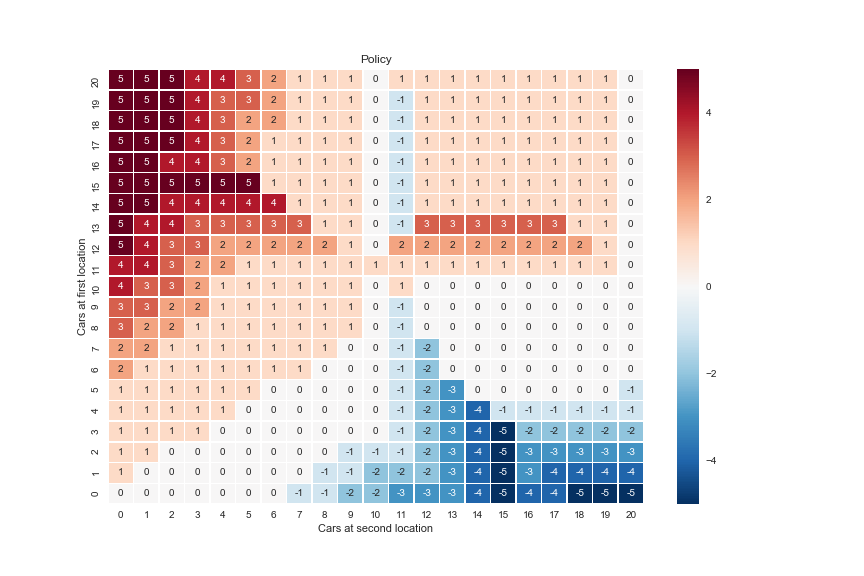
\includegraphics[scale=0.75]{policy_4_7.png}
	\label{fig:policy_4_7}
\end{figure}

\begin{figure}[h]
	\centering
	\caption{Optimal value function for Exercise 4.7}
	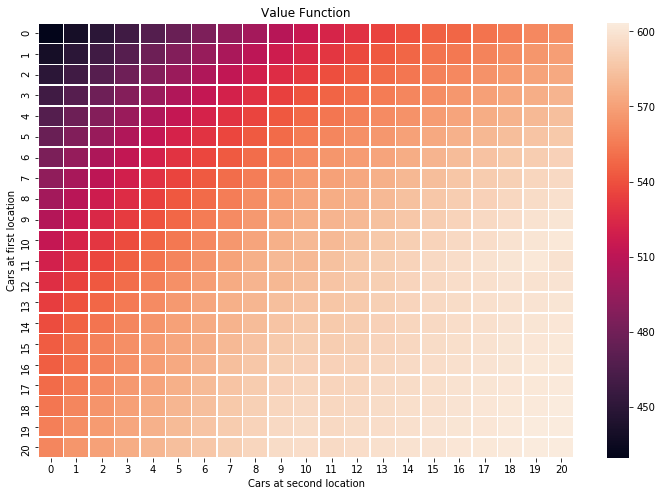
\includegraphics[scale=0.75]{value_function_4_7.png}
	\label{fig:value_function_4_7}
\end{figure}


\section{Exercise 4.8}

\textbf{Why does the optimal policy for the gambler’s problem have such a curious form? In particular, for capital of 50 it bets it all on one flip, but for capital of 51 it does not. Why is this a good policy?}
\\ \\
Assume that the value of all states are initialised as 0, except $s=100$ for which the value is 1. Assume also that we sweep through the states in increasing order. As $s=100$ cannot be reached from any state less than 50, the values of all states less than 50 will remain 0 during the first sweep. For $s=50$, the only action with non-zero value with respect to the initial value function is $a=50$, so $V(50)$ will be set to $0.4 \cdot 1 + 0.6 \cdot 0 = 0.4$.
\\ \\
Now for $s=51$ there are two actions with non-zero value, $a=49$ and $a=1$. The value of $a=49$ is $0.4$ and the value of $a=1$ is 
\[
	0.4 (0 + V(52)) + 0.6 (0 + V(50)) = 0.6 \cdot 0.4 = 0.24.
\]
Thus, $a=49$ is the maximising action and $V(51)$ will be set to $0.4$. Similarly, $V(s)$ will be set to $0.4$ during the first sweep for all $s=52, 53, \dots, 74$.
\\ \\
Now consider $s=75$. From here the gambler can reach 100 and, failing that, fall back to 50, which also has non-zero value. The maximising action is $a=25$ with value 
\[
	0.4 \cdot  V(100) + 0.6 \cdot  V(50) = 0.4 \cdot 1 + 0.6 \cdot 0.4 = 0.64.
\]
The same is true for $s=76, 77, \dots, 87$.
\\ \\
Now consider $s=88$. From here the gambler can reach 100 and, failing that, fall back to 76, whose value is greater than 50. The maximising action is $a=12$ with value 
\[
0.4 \cdot  V(100) + 0.6 \cdot  V(76) = 0.4 \cdot 1 + 0.6 \cdot 0.64 = 0.784.
\]
The same is true for $s=89, 90, \dots, 93$.
\\ \\
Now we start to see a pattern emerging. In the long run we imagine that the gambler learns to use these intermediate values where we see peaks in the policy graph (13, 25, 38, 50, 63, 75, 88) as \emph{stepping stones} (looking forward) and \emph{safety nets} (looking back), with the goal of ultimately reaching \$100. 




%For capitals of $s=52, \dots, 99$, betting $s - 50$ is again preferable to betting $s$, but perhaps we can do better. Suppose that the gambler's capital is $63$. Here he could bet  
%
%We could argue similarly for capitals of 52 to 99
%
%We can argue similarly for capitals of $52, 53, \dots, 62$.
%
%Now when he has capital of $63$, if he bets 


\section{Exercise 4.9}

The optimal policy and value function for $p_h = 0.25$ are shown in Figures \ref{fig:policy_4_9_ph_25} and \ref{fig:value_4_9_ph_25} respectively. The optimal policy and value function for $p_h = 0.55$ are shown in Figures \ref{fig:policy_4_9_ph_55} and \ref{fig:value_4_9_ph_55} respectively.
For $p_h = 0.25$, the policy changes for different values of $\theta$ as $\theta \rightarrow 0$. However, for $p_h = 0.55$ the policy is stable as $\theta \rightarrow 0$, which suggests that the optimal policy of always betting \$1 is in fact unique.

\begin{figure}
	\centering
	\caption{Optimal policy for Exercise 4.9 with $p_h = 0.25$}
	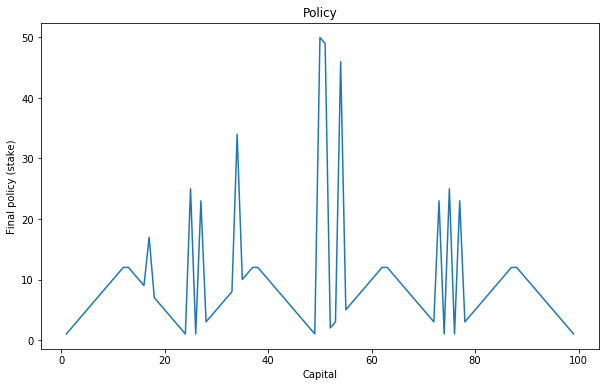
\includegraphics[scale=0.75]{policy_4_9_ph_25.png}
	\label{fig:policy_4_9_ph_25}
\end{figure}

\begin{figure}
	\centering
	\caption{Optimal value function for Exercise 4.9 with $p_h = 0.25$}
	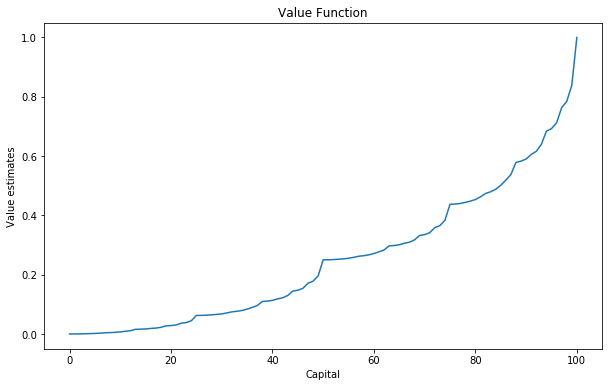
\includegraphics[scale=0.75]{value_4_9_ph_25.png}
	\label{fig:value_4_9_ph_25}
\end{figure}

\begin{figure}
	\centering
	\caption{Optimal policy for Exercise 4.9 with $p_h = 0.55$}
	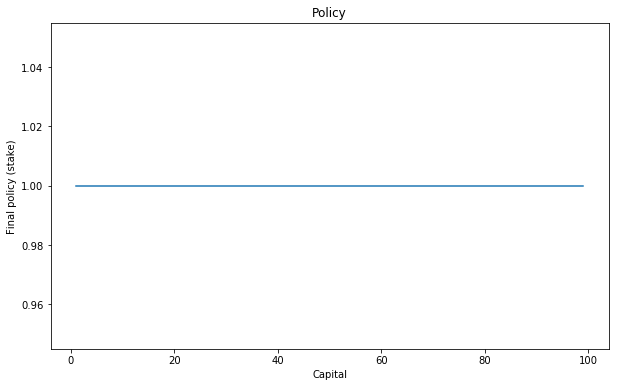
\includegraphics[scale=0.75]{policy_4_9_ph_55.png}
	\label{fig:policy_4_9_ph_55}
\end{figure}

\begin{figure}
	\centering
	\caption{Optimal value function for Exercise 4.9 with $p_h = 0.55$}
	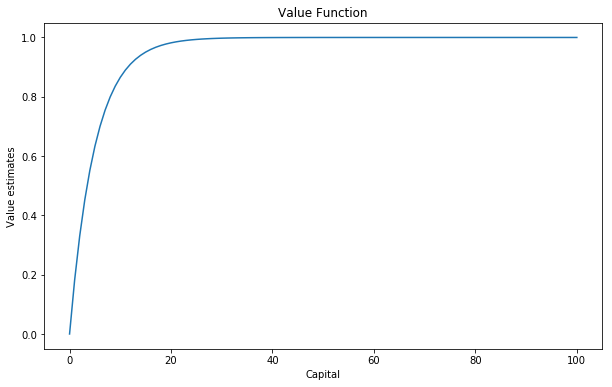
\includegraphics[scale=0.75]{value_4_9_ph_55.png}
	\label{fig:value_4_9_ph_55}
\end{figure}



\section{Exercise 4.10}

\textbf{What is the analog of the value iteration update (4.10) for action values, $q_{k+1}(s, a)$?}
\\ \\
The update is
\begin{align*}
	q_{k+1}(s, a) = \sum_{s', r} p(s', r | s, a) \Big [r + \gamma \max_{a'} q_{k}(s', a') \Big].
\end{align*}


\end{document}